\graphicspath{{5perm/asy/},{8action/asy/}}

\section{Group Actions}\label{chap:action}


\subsection{Group Actions, Fixed Sets and Isotropy Subgroups}\label{sec:action1}

In this final chapter, we revisit a central idea: groups are interesting and useful often because of how they \emph{transform sets.} Recall how the symmetric group $S_n$ was defined in terms of what its elements do to the set $\{1,\ldots,n\}$. This is an example of a general situation.

\begin{defn}{}{}
A group $G$ \emph{acts\footnotemark} on a set $X$ via a map $\cdot:G\times X\to X$ if,
\begin{enumeratea}
  \item $\forall x\in X,\ e\cdot x=x$,\quad and,
  \item $\forall x\in X,\ g,h\in G,\  g\cdot (h\cdot x)=(gh)\cdot x$.
\end{enumeratea}
\end{defn}

\footnotetext{This is really a \emph{left} action. There is an analogous definition of a \emph{right action.} In this course, all actions will be left.}

Part (b) says $g\mapsto g\cdot$ is a homomorphism of \emph{binary structures} (the functions $X\to X$ needn't form a group).

\begin{examples}{}{actioneasy}
\exstart The symmetric $S_n$ group acts on $X=\{1,2,\ldots,n\}$. As a sanity check:\vspace{-3pt}
\begin{enumerate}\setcounter{enumi}{1}
  \item[]\begin{enumerate}
		\item $e(x)=x$ for all $x\in \{1,\ldots,n\}$.
		\item $\sigma\bigl(\tau(x)\bigr)=(\sigma\tau)(x)$ is composition of functions!
	\end{enumerate}
  \item Any group $G$ acts on itself by left multiplication. This is essentially Cayley's Theorem (\ref{thm:cayley}). It also acts on itself by conjugation ($c_g\circ c_h=c_{gh}$ is Theorem \ref{thm:aut}).
  \item If $X$ is the set of orientations of a regular $n$-gon such that one vertex is at $(1,0)$ and the center is at $(0,0)$, then $D_n$ acts on $X$ by rotations and reflections. Note that $X$ has cardinality $2n$.
  \item Matrix groups act on vector spaces by matrix multiplication. For example the orthogonal group $\rO_2(\R)$ can be seen to transform vectors via rotations and reflections.
	\[\rO_2(\R)\times\R^2\to\R^2:(A,\vv)\mapsto A\vv\]
  
  \item\label{ex:orthmultaction} A group can act on many different sets. Here are three further actions of the orthogonal group:
	\begin{enumerate}
  	\item[i.] $\rO_2(\R)$ acts on the set $X=\{1,-1\}$ via $A\cdot x:=(\det A)x$.
		\item[ii.] $\rO_2(\R)$ acts on the set $X=\R^3$ via $A\cdot\vv:=A(v_1\vi+v_2\vj)+v_3\vk$.
		\item[iii.] $\rO_2(\R)$ acts on the unit circle $X=S^1\subseteq\R^2$ via matrix multiplication $A\cdot\vv:=A\vv$.
	\end{enumerate}
\end{enumerate}
\end{examples}

We often use an action to visualize a group; in this context, some actions are better than others. Consider the three actions of $\rO_2(\R)$ in part \ref*{ex:orthmultaction} above:
\begin{enumerate}\itemsep0pt
  \item[i.] The set $X$ is very small. Many matrices act in exactly the same way so the action is an unhelpful means of visualizing the group.
	\item[ii.] The set $X$ feels too large. The action leaves any vertical vector untouched.
	\item[iii.] The circle $X=S^1$ is large enough so that the action of distinct matrices can be distinguished without being inefficiently large.\footnote{A \emph{Goldilocks} action, perhaps?}
\end{enumerate}

\goodbreak

These notions can be formalized.



\begin{defn}{}{}
Let $G\times X\to X$ be an action.
\begin{enumerate}
  \item The \emph{fixed set} of $g\in G$ is the set
  \[\Fix(g):=\{x\in X:g\cdot x=x\} \tag{also written $X_g$, though we won't do this}\]
  \item The \emph{isotropy subgroup} or \emph{stabilizer} of $x\in X$ is the set
  \[\Stab(x):=\{g\in G:g\cdot x=x\} \tag{also written $G_x$}\] 
  \item The action is \emph{faithful} if the only element of $G$ which fixes everything is the identity. This can be stated in two equivalent ways:
  \begin{enumerate}
    \item $\Fix(g)=X\iff g=e$\qquad\qquad\qquad (b)\lstsp$\bigcap\limits_{x\in X}\Stab(x)=\{e\}$
  \end{enumerate}
  \item The action is \emph{transitive} if any element of $X$ may be transformed to any other:
	\[\forall x,y\in X,\ \exists g\in G\ \text{ such that }\  y=g\cdot x\]
\end{enumerate}
\end{defn}

\begin{examples*}{\ref{ex:actioneasy} cont}{}
\exstart The action of $S_n$ on $\{1,2,\ldots,n\}$ is both faithful and transitive:
\begin{enumerate}\setcounter{enumi}{1}
  \item[]\begin{description}
  	\item[\normalfont\emph{Faithful}:] if $\sigma(x)=x$ for all $x\in\{1,2,\ldots,n\}$, then $\sigma=e$.
  	\item[\normalfont\emph{Transitive}:] if $x\neq y$, then the 2-cycle $(x\,y)$ maps $x\mapsto y$.
  \end{description}
  \item The action of a group on itself by left multiplication is both faithful and transitive. Conjugation is more complex: in most situations it is neither.
  \item $D_n$ acts faithfully and transitively on the orientations of the $n$-gon.
  \item The action of $\rO_2(\R)$ on $\R^2$ is faithful but not transitive: for instance the zero vector cannot be transformed into any other vector so $\Stab(\V0)=\rO_2(\R)$.
  \item We leave these as exercises.
%   \begin{enumerate}
%     \item[i.] The action $A\cdot x=\det(A)x$ is transitive, but not faithful: indeed if $A$ is any orthogonal matrix with determinant 1, then $\Fix(A)=X$.
%     \item[ii.] The action of $\rO_2(\R)$ on $\R^3$ is faithful but not transitive. It is impossible to transform, say, the zero vector into anything else.
%     \item[iii.] The action of $\rO_2(\R)$ is both faithful and transitive.
% 	\end{enumerate}
\end{enumerate}
\end{examples*}


\begin{lemm}{}{}
For each $x\in X$, the stabilizer $\Stab(x)$ is indeed a subgroup of $G$.
\end{lemm}

\begin{proof}
$\Stab(x)$ is a non-empty subset of $G$ since $e\in \Stab(x)$. It sufficient to show that it is closed under multiplication and inverses. Let $g,h\in\Stab(x)$, then
\[(gh)\cdot x=g\cdot(h\cdot x)=g\cdot x=x\implies gh\in\Stab(x)\]
Moreover
\[x=g\cdot x\implies g^{-1}\cdot x=g^{-1}\cdot (g\cdot x)=(g^{-1}g)\cdot x=e\cdot x=x\tag*{\qedhere}\]
\end{proof}

\begin{example}{}{actiond3}
The dihedral group $D_3=\{e,\rho_1,\rho_2,\mu_1,\mu_2,\mu_3\}$ acts on the set $X$ of vertices of an equilateral triangle.\footnotemark\ The fixed sets and stabilizers for this action are as follows:\par
\begin{minipage}[t]{0.74\linewidth}\vspace{-10pt}
\[\begin{array}[t]{c|c}
\text{Element $g$}&\Fix(g)\\\hline
e&\{1,2,3\}\\
\rho_1&\emptyset\\
\rho_2&\emptyset\\
\mu_1&\{1\}\\
\mu_2&\{2\}\\
\mu_3&\{3\}
\end{array}
\qquad
\begin{array}[t]{c|c}
\text{Vertex $x$}&\Stab(x)\\\hline
1&\{e,\mu_1\}\\
2&\{e,\mu_2\}\\
3&\{e,\mu_3\}
\end{array}\]
\end{minipage}\hfill\begin{minipage}[t]{0.25\linewidth}\vspace{-20pt}
\flushright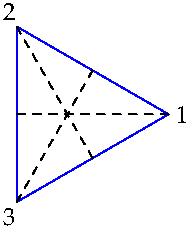
\includegraphics{perm-d3}
\end{minipage}\smallbreak
$D_3$ also acts on the set of \emph{edges} of the triangle $Y=\bigl\{\{1,2\},\{1,3\},\{2,3\}\bigr\}$. You needn't write all these out since, by the symmetry of the triangle, stabilizing an edge is equivalent to stabilizing its opposite vertex. Still, here is the data:
\[\begin{array}[t]{c|c}
\text{Element $g$}&\Fix(g)\\\hline
e&\bigl\{1,2,3\bigr\}\\
\rho_1&\emptyset\\
\rho_2&\emptyset\\
\mu_1&\bigl\{\{2,3\}\bigr\}\\
\mu_2&\bigl\{\{1,3\}\bigr\}\\
\mu_3&\bigl\{\{1,2\}\bigr\}
\end{array}
\qquad
\begin{array}[t]{c|c}
\text{Edge $\{x,y\}$}&\Stab(\{x,y\})\\\hline
\{1,2\}&\{e,\mu_3\}\\
\{1,3\}&\{e,\mu_2\}\\
\{2,3\}&\{e,\mu_1\}
\end{array}\]
\end{example}

\footnotetext{Recall that $\rho_1$ rotates \ang{120} counter-clockwise, that $\rho_2=\rho_1^2$ and that $\mu_i$ reflects across the altitude through vertex $i$.}



\begin{exercises}{}{}
Key concepts:
\begin{quote}
	\emph{(left) action\quad $\Fix(g)$\quad $\Stab(x)\le G$\quad faithful/transitive actions}
\end{quote}

\begin{enumerate}
  \item For part \ref*{ex:orthmultaction} of Example \ref{ex:actioneasy}, determine whether each action is faithful and/or transitive.

	
	\item\label{exs:orbitsigma1} Let $G=\ip{\sigma}\le S_6$ where $\sigma=(1\,2\,3\,4\,5\,6)$. $G$ acts on the set $X=\{1,2,3,4,5,6\}$ in a natural way.
	\begin{enumerate}
	  \item State the fixed sets and stabilizers for this action.
	  \item Is the action of $G$ faithful? Transitive?
	\end{enumerate}
	
	
	\item\label{exs:orbitsigma2} Repeat the previous question when $\sigma=(1\,3)(2\,4\,6)$.
	

	\item Mimic Example \ref{ex:actiond3} for the actions of $D_4$ on $X=\{$vertices$\}$ and $Y=\{$edges$\}$ of the square.\\
	(\emph{Use whatever notation you like; $\rho,\mu,\delta$ or cycle notation})


	\item Suppose $G$ acts on $X$.
	\begin{enumerate}
	  \item Let $Y\subseteq X$ and define $\Stab Y=\{g\in G:\forall y\in Y, g\cdot y=y\}$. Prove that $\Stab Y$ is a subgroup of $G$.
		\item Let $G$ act on itself by conjugation ($X=G$!). What is another name for the subgroup $\Stab G$?
	\end{enumerate}
	

	\item Suppose $G$ has a left action on $X$. Prove that $G$ acts faithfully on $X$ if and only if no two distinct elements of $G$ have the same action on every element.

\end{enumerate}
\end{exercises}

\clearpage



\subsection{Orbits \& Burnside's Formula}

We first encountered orbits in the context of the symmetric groups $S_n$. The same idea applies to any action.

\begin{defn}{}{}
Let $G\times X\to X$ be an action. The \emph{orbit} of $x\in X$ under $G$ is the set of elements into which $x$ may be transformed:
\[Gx=\{g\cdot x:g\in G\}\subseteq X\]
\end{defn}


\begin{examples}{}{}
\exstart If $X=\{1,2,\ldots n\}$ and $G=\ip{\sigma}\le S_n$, then
\[Gx=\{\sigma^k(x):k\in\Z\}=\orb_x(\sigma)\]
The definition of orbits therefore coincides with that seen earlier in the course.
\begin{enumerate}\setcounter{enumi}{1}
  \item A transitive \emph{action\footnotemark} has only one orbit.
  
  \item If $\rO_2(\R)$ acts on $\R^2$ by matrix multiplication, then the orbits are circles centered at the origin!
\end{enumerate}
\end{examples}

\footnotetext{Unhelpfully, we now have two meanings of \emph{transitive}; one for equivalence relations and one for actions.}


\begin{lemm}{}{actionorbit}
The orbits of an action partition $X$.
\end{lemm}

Since this is almost identical to the corresponding result for orbits in $S_n$ (Theorem \ref{thm:orbit}), we leave the proof as an exercise.


\smallbreak
Our next result is analogous to Lemma \ref{lemm:homobij}, where we counted the number of (left) cosets of $\ker\phi$.

% \begin{proof}
% Define $x\sim y\iff y\in Gx\iff \exists g\in G$ such that $g\cdot x=y$. We claim that $\sim$ is an equivalence relation.
% \begin{description}
% 	\item[\normalfont\emph{Reflexivity}:] $x=e\cdot x\implies x\sim x$.
% 	\item[\normalfont\emph{Symmetry}:] $g\cdot x=y\implies x=g^{-1}\cdot y$, thus $x\sim y\implies y\sim x$.
% 	\item[\normalfont\emph{Transitivity}:] If $x\sim y$ and $y\sim z$, then $y=g\cdot x$ and $z=h\cdot y$ for some $g,h\in G$. But then $z=(hg)\cdot x$, whence $x\sim z$.\qedhere
% \end{description}
% \end{proof}



\begin{lemm}{}{actionorbits2}
The cardinality of the orbit $Gx$ is the index of the isotropy subgroup $\Stab(x)$:
\[\nm{Gx}=\bigl(G:\Stab(x)\bigr)\]
\end{lemm}


\begin{proof}
Observe that
\[g\cdot x=h\cdot x\iff h^{-1}g\cdot x=x\iff h^{-1}g\in \Stab(x)\iff g\Stab(x)=h\Stab(x)\]
The contrapositive says that distinct elements of the orbit $Gx$ correspond to distinct left cosets.
\end{proof}


\begin{example}{}{burnsimple}
 Let $\sigma=(1\,4)(2\,7\,3)\in S_7$. Consider $X=\{1,2,3,4,5,6,7\}$ under the action of the cyclic group $G=\ip{\sigma}$. The orbits are precisely the disjoint cycles: $\{1,4\}$, $\{2,3,7\}$, $\{5\}$, $\{6\}$. Observe that $G$ has six elements:
\[e,\quad \sigma=(1\,4)(2\,7\,3),\quad \sigma^2=(2\,3\,7),\quad \sigma^3=(1\,4),\quad \sigma^4=(2\,7\,3),\quad \sigma^5=(1\,4)(2\,3\,7)\]
The Lemma is easily verifiable: for instance if $x=3$,
\begin{gather*}
\Stab(x)=\{\tau\in G:\tau(3)=3\}=\{\sigma^k:\sigma^k(3)=3\}=\{e,\sigma^3\}\\
\implies (G:\Stab(x))=\frac 62=3=\nm{\{2,3,7\}}=\nm{Gx}
\end{gather*}
\end{example}


% \boldsubsubsection{Burnside's formula}
% 
It is often useful to count the \emph{number} of orbits of an action. For \emph{finite} actions, this turns out to be possible in two different ways.

\begin{thm}{Burnside's formula}{}
Let $G$ be a finite group acting on a finite set $X$. Then the number of orbits in $X$ under $G$ satisfies
\[\text{\# orbits}=\frac{1}{\nm G}\sum_{x\in X}\nm{\Stab(x)}=\frac{1}{\nm G}\sum_{g\in G}\nm{\Fix(g)}\]
\end{thm}

\begin{proof}
By Lemma \ref{lemm:actionorbits2},
It follows that
\[\frac 1{\nm G}\sum_{x\in X}\nm{\Stab(x)} =\sum_{x\in X}\frac{\nm{\Stab(x)}}{\nm G} =\sum_{x\in X}\frac 1{(G:\Stab(x))} =\sum_{x\in X}\frac{1}{\nm{Gx}}.\tag*{($\ast$)}\]
Consider a fixed orbit $Gy$. Since $\nm{Gx}=\nm{Gy}$ for each $x\in Gy$, we see that
\[\sum_{x\in Gy}\frac{1}{\nm{Gx}}=\frac{\nm{Gy}}{\nm{Gy}}=1\]
The sum ($\ast$) therefore counts 1 for each distinct orbit in $X$ and therefore returns the number of orbits.\smallbreak
For the second equality, observe that
\[S=\{(g,x)\in G\times X:g\cdot x=x\}\]
has cardinality
\[\nm S=\sum\limits_{x\in X}\nm{\Stab(x)}=\sum\limits_{g\in G}\nm{\Fix(g)}\tag*{\qedhere}\]
\end{proof}



\begin{example*}{\ref{ex:burnsimple} cont}{}
When $G=\ip\sigma=\ip{(1\,4)(2\,7\,3)}$ acts on $X=\{1,2,3,4,5,6,7\}$, the stabilizers and fixed sets are as follows:
	\[\begin{array}{c|c}
	x\in X&\Stab(x)\\\hline
	1&\{e,\sigma^2,\sigma^4\}\\
	2&\{e,\sigma^3\}\\
	3&\{e,\sigma^3\}\\
	4&\{e,\sigma^2,\sigma^4\}\\
	5&G=\{e,\sigma,\sigma^2,\sigma^3,\sigma^4,\sigma^5\}\\
	6&G\\
	7&\{e,\sigma^3\}
	\end{array}\qquad\qquad\begin{array}{c|c}
	g\in G&\Fix(g)\\\hline
	e&X=\{1,2,3,4,5,6,7\}\\
	\sigma&\{5,6\}\\
	\sigma^2&\{1,4,5,6\}\\
	\sigma^3&\{2,3,5,6,7\}\\
	\sigma^4&\{1,4,5,6\}\\
	\sigma^5&\{5,6\}\\
	\multicolumn{2}{c}{}
	\end{array}\]
	Burnside's formula just sums the number of elements in all of the subsets in the right column of each table:
\begin{align*}
4=\text{\# orbits}&=\frac{1}{\nm G}\sum_{x\in X}\nm{\Stab(x)}=\frac{1}{6}(3+2+2+3+6+6+2)\\
&=\frac{1}{\nm G}\sum_{g\in G}\nm{\Fix(g)}=\frac{1}{6}(7+2+4+5+4+2)
\end{align*}
\end{example*}

\goodbreak

One reason to count the number of orbits of an action is that we often want to consider objects as equivalent if they differ by the action of some simple group.

\begin{example}{}{toy}
A child's toy consists of a wooden equilateral triangle where the edges are to be painted using any choice of colors from the rainbow. How many distinct toys could we create?\smallbreak
There are two problems: we need to describe the variety of possible toys, and we need to know what \emph{distinct} means!\smallbreak
We use group actions to address both problems:
\begin{itemize}
  \item A toy may be considered as a subset of $X=\{$painted triangles$\}=\{$ordered color triples$\}$. Since there are 7 choices for the color of each edge, we see that $\nm X=7^3=343$ is a large set!
\begin{minipage}[t]{0.55\linewidth}\vspace{0pt}
  \item Two toys are equivalent if they differ by a rotation in 3-dimensions. This amount to the natural action of $D_3$ on $X$: for instance
  \[\rho_1\cdot (\text{red,green,violet})=(\text{violet,red,green})\]
\end{minipage}\hfill\begin{minipage}[t]{0.4\linewidth}\vspace{0pt}
\hfill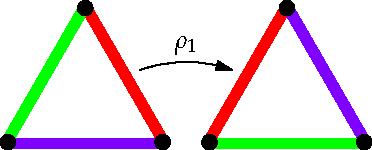
\includegraphics{actions-triangles}
\end{minipage}
\end{itemize}
The number of orbits is the number of distinct toys, which we may compute using Burnside. Since it would be time consuming to compute the stabilizer of each element of $X$, we use the fixed set approach.
\begin{itemize}
  \item Identity $e$: \ Plainly $\Fix(e)=X$, since $e$ leaves every coloring unchanged.
  \item Rotations $\rho_1,\rho_2$: \ If a color-scheme is fixed by $\rho_j$, then all pairs of adjacent edges must be the same color. The only color-schemes fixed by $\rho_j$ are those where all sides have the same color, whence $\nm{\Fix(\rho_i)}=7$.
  \item Reflections $\mu_1,\mu_2,\mu_3$: \ Since $\mu_j$ swaps two edges, anything in its fixed set must have these edges the same. We have 7 choices for the color of the switched edges, and an independent choice of 7 colors for the other edge, whence $\nm{\Fix(\mu_j)}=7^2=49$.
\end{itemize}
The number of distinct toys is therefore
\begin{align*}
\text{\# orbits}&=\frac 1{\nm{D_3}}\sum_{\sigma\in D_3}\nm{\Fix(\sigma)}=\frac 16(7^3+7+7+7^2+7^2+7^2)\\
&=\frac 76(49+1+1+7+7+7)=84
\end{align*}
The question was a little tricky because we are allowed multiple sides to have the same color. A simpler version would restrict to the situation where all sides had to be different colors. In this case $D_3$ acts on a set of color schemes with cardinality $\nm Y=7\cdot 6\cdot 5=210$. Moreover, only the identity element has a non-empty fixed set; in this situation the number of distinct toys would be
\[\text{\# orbits}=\frac 1{\nm{D_3}}\sum_{\sigma\in D_3}\nm{\Fix(g)}=\frac 16(210+0+\cdots+0)=\frac{210}6=35\]
Of course you could answer these questions by pure combinatorics without any resort to group theory!
\end{example}

\goodbreak

\boldsubsubsection{Dice-rolling for Geeks!}

\begin{minipage}[t]{0.69\linewidth}\vspace{-10pt}
Games like Dungeons \& Dragons make use of several differently shaped dice: rather than simply using the standard 6-sided cubic die, situations might require rolling, say, a 4-sided tetrahedral die or a 20-sided icosahedral die.\smallbreak
Since dice are designed for rolling, we consider two dice to be the same if one can be rotated into the other. Play with the two tetrahedral dice on the right; you should be convinced that you cannot rotate one to make the other so these dice are distinct.\smallbreak
It is not difficult to see that, up to rotations, these are the \emph{only} tetrahedral dice just by counting!
\begin{itemize}
  \item Place face 4 on the table.
  \item When looking from above, the remaining faces are numbered 1, 2, 3 either clockwise or counter-clockwise. 
\end{itemize}
For larger dice, this approach is not practical! However, with a little thinking about symmetry groups, Burnside's formula will ride to the rescue.\smallbreak
Suppose a regular polyhedron has $f$ faces, each with $n$ sides.
\end{minipage}\hfill\begin{minipage}[t]{0.3\linewidth}\vspace{-20pt}
\flushright
	\href{https://www.math.uci.edu/~ndonalds/math120a/perm-a4.html}{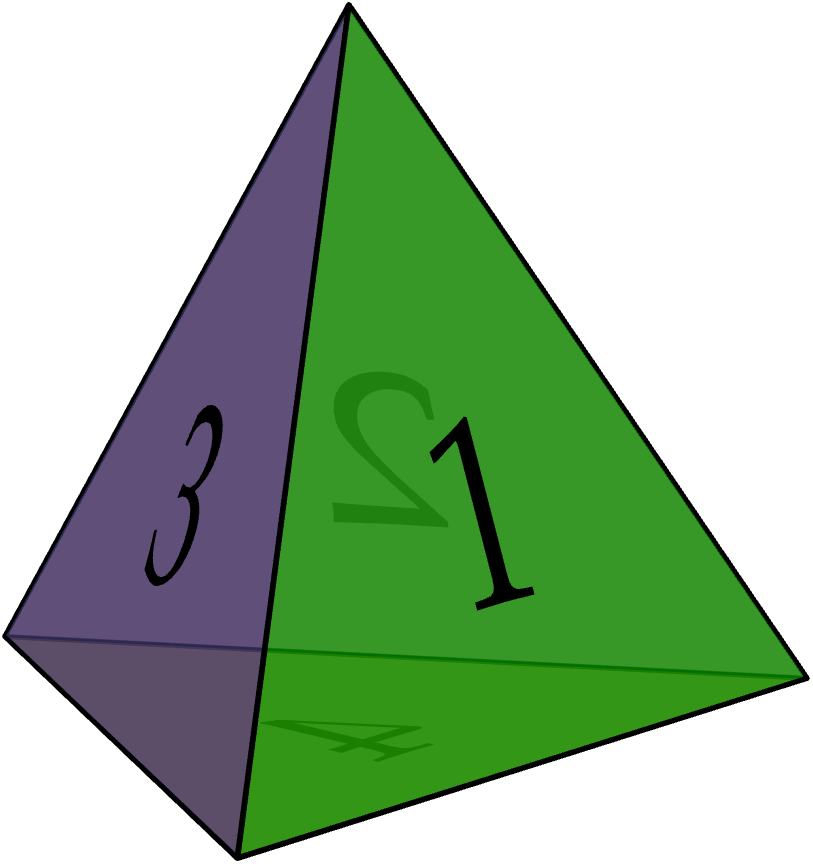
\includegraphics[scale=0.15]{perm-a4.png}}\bigbreak
  \href{https://www.math.uci.edu/~ndonalds/math120a/actions-a4-2.html}{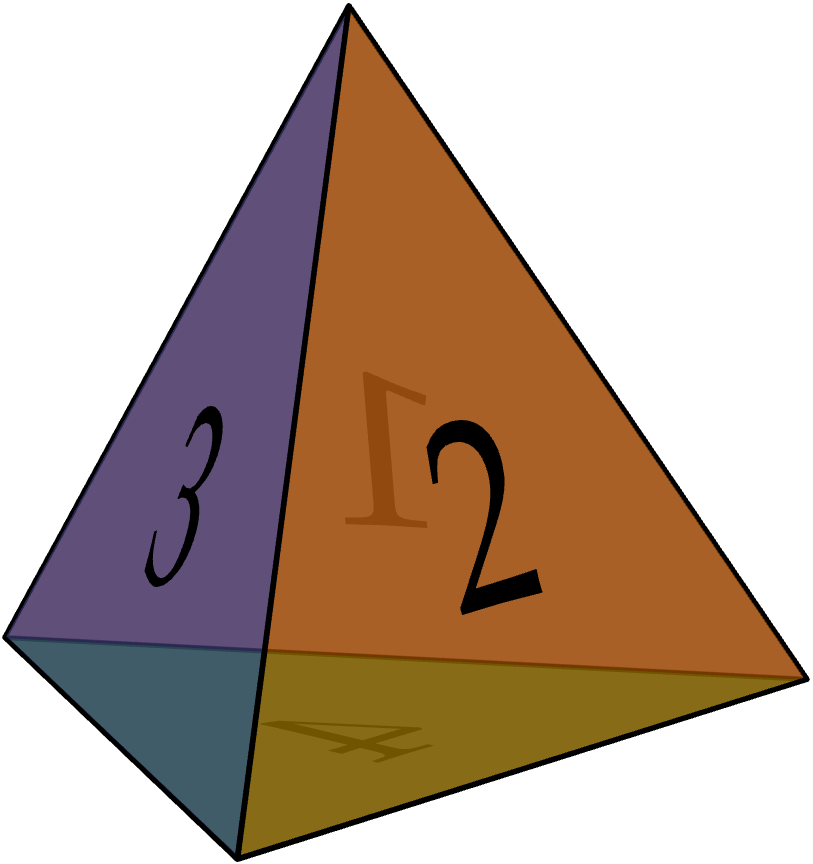
\includegraphics[scale=0.15]{actions-a4-2.png}}
\end{minipage}\par

\begin{itemize}
  \item The faces may be labelled 1 thorough $f$ in $f!$ distinct ways: the set of distinct labellings is $X$.
  \item We may rotate the polyhedron so that any face is mapped to any other, \emph{in any orientation.} It follows that the rotation group $G$ has $fn$ elements.
	\item Each non-identity element of the rotation group moves at least one face, whence
	\[\nm{\Fix(g)}=\begin{cases}
	X&\text{if }g=e\\
	\emptyset&\text{if }g\neq e
	\end{cases}\]
	\item The number of distinct dice for a regular polyhedron is therefore
	\[\text{\# orbits}=\frac 1{\nm G}\nm{\Fix(e)}=\frac{\nm X}{\nm G}=\frac{f!}{fn}=\frac{(f-1)!}{n}\]
	We don't need to know what the rotation group is, only its \emph{order}. For completeness, here are all the possibilities for the regular platonic solids.
	\begin{quote}
	\begin{tabular}{l|c|c|c|l}
		Polyhedron & $f$ & $n$ & Rotation Group & $\#$ distinct dice\\\hline
		Tetrahedron & 4 & 3 & $A_4$ & 2\\
		Cube & 6 & 4 & $S_4$ & 30\\
		Octahedron & 8 & 3 &  $S_4$ & 1,680\\
		Dodecahedron & 12 & 5 & $A_5$ & 7,983,360\\
		Icosahedron & 20 & 3 & $A_5$ & 40,548,366,802,944,000
	\end{tabular}
	\end{quote}
\end{itemize} 


\goodbreak

\boldsubsubsection{Subgroups of Prime Order \& the Class Equation}

We finish with a taste of where group theory traditionally goes next.\smallbreak

Suppose $G$ acts on a finite set $X$, that $x_1\ldots,x_r$ are representatives of the distinct orbits and that $x_1,\ldots,x_s$ enumerate the 1-element orbits ($\Stab(x_j)=G \iff j\le s$). Then, by counting elements,
\[\nm X=s+\sum_{j=s+1}^r\nm{Gx_j} =s+\sum_{j=s+1}^r\bigl(G:\Stab(x_j)\bigr)\]
When $G$ acts on itself by conjugation, the 1-element orbits together comprise the center of $G$ and we obtain the \emph{class equation}:
\[\nm{G}=\nm{Z(G)}+\sum_{j=s+1}^r \bigl(G:\Stab(x_j)\bigr)\]

\begin{example}{}{}
Since the conjugacy classes in $S_4$ are the cycle types, the class equation reads
\begin{align*}
24&=\nm{\{e\}} +\nm{\text{2-cycles}} +\nm{\text{3-cycles}} +\nm{\text{4-cycles}} +\nm{\text{2,2-cycles}} %=1+\binom 42+2\binom 43+3!+3\\
=1+6+8+6+3
\end{align*}
\end{example}

Here is an example of how the class equation may be applied.

\begin{lemm}{}{}
Suppose $G$ is a non-abelian group whose order is divisible by a prime $p$. Then $G$ has a \emph{proper} subgroup whose order is divisible by $p$.
\end{lemm}

\begin{proof}
Since $G$ is non-abelian, $Z(G)$ is a proper subgroup. Let $x$ be any element \emph{not} in the center. Then
	\[2\le \nm{Gx}=\frac{\nm G}{\nm{\Stab(x)}} \implies \Stab(x)\text{ is a proper subgroup of }G\]
	If $p$ divides $\nm{\Stab(x)}$, then we're done. If not, then $p$ divides $\nm{Gx}=\bigl(G:\Stab(x)\bigr)$. If this holds for all non-trivial orbits, the class equation says that $\nm{Z(G)}$ is divisible by $p$.
\end{proof}

%The Lemma can be used as part of an induction process to prove a famous result.

\begin{thm}{Cauchy}{}
If a prime $p$ divides $\nm G$, then $G$ contains a subgroup/element of order $p$. 
\end{thm}

\footnotetext{The two are equivalent: if $y$ has order $p$, then $\ip{y}$ is a subgroup of order $p$. If $H\le G$ has order $p$, then $H\cong \Z_p$ is cyclic.}

It might feel as if we've done this already; Exercise \ref*{chap:direct}.\ref{exs:abeliansubgroup} covers abelian groups, but this depends on the fundamental theorem, which first requires Cauchy for abelian groups! 



\begin{proof}
\begin{enumerate}
  \item A proof for when $G$ is abelian is in the exercises.
  \item If $G$ is non-abelian, apply the Lemma. If the resulting subgroup is abelian, part 1 finishes things off. Otherwise repeat. If we never reach an abelian subgroup, then we have an infinite sequence of proper subgroups and thus a decreasing sequence of positive integers; contradiction.\qedhere
\end{enumerate}
\end{proof}

Cauchy's Theorem may be extended to prove that if $p^k$ divides $G$, then $G$ has a subgroup of order $p^k$. This is the beginning of the Sylow theory of $p$-subgroups which has applications to group classification and the existence of sequences of normal subgroups. 


\goodbreak

\begin{exercises}{}{}
Key concepts:
\begin{quote}
\emph{Orbits of $G$ partition $X$\qquad Cardinality of orbit $\nm{Gx}=(G:\Stab(x))$ divides $\nm G$\\
Burnside's formula for counting number of orbits}
\end{quote}

\begin{enumerate}
  \item Determine the orbits of $G=\ip\sigma$ on $X=\{1,2,3,4,5,6\}$ for each of Exercises \ref*{sec:action1}.\ref{exs:orbitsigma1} and \ref{exs:orbitsigma2}. In both cases verify Burnside's formula.
  
  
	\item Revisit Example \ref{ex:toy}. How may distinct toys may be created if:
	\begin{enumerate}
	  \item A maximum of two colors can be used?
	  \item Exactly two colors must be used?
	\end{enumerate}
	
  
  \item Prove Lemma \ref{lemm:actionorbit}: the orbits of a left action partition $X$.
  
	
	\item A 10-sided die is shaped so that all faces are congruent \emph{kites}: five faces are arranged around the north pole and five around the south, so that each face is adjacent to four others.
	\begin{enumerate}
	  \item Argue that the group of rotational symmetries of such a die has ten elements.\par
	  (\emph{In fact it is non-abelian and is therefore isomorphic to $D_5$}).
	  \item Use Burnside's formula to determine how many distinct 10-sided dice may be produced.
	\end{enumerate}
	




	\begin{minipage}[t]{0.74\linewidth}\vspace{-6pt}
		\item A soccer ball is constructed from 20 regular hexagons and 12 regular pentagons as in the picture.\par
		Suppose the 20 hexagonal patches are all to have different colors, as are the 12 pentagonal patches. How many distinct balls may be produced?
		
		\item The faces of a cuboid measuring $1\times 1\times 2$\,in is to be painted using (at most) two colors. Up to equivalence by rotations, how many ways can this be done? 
	\end{minipage}\hfill\begin{minipage}[t]{0.25\linewidth}\vspace{-25pt}
		\flushright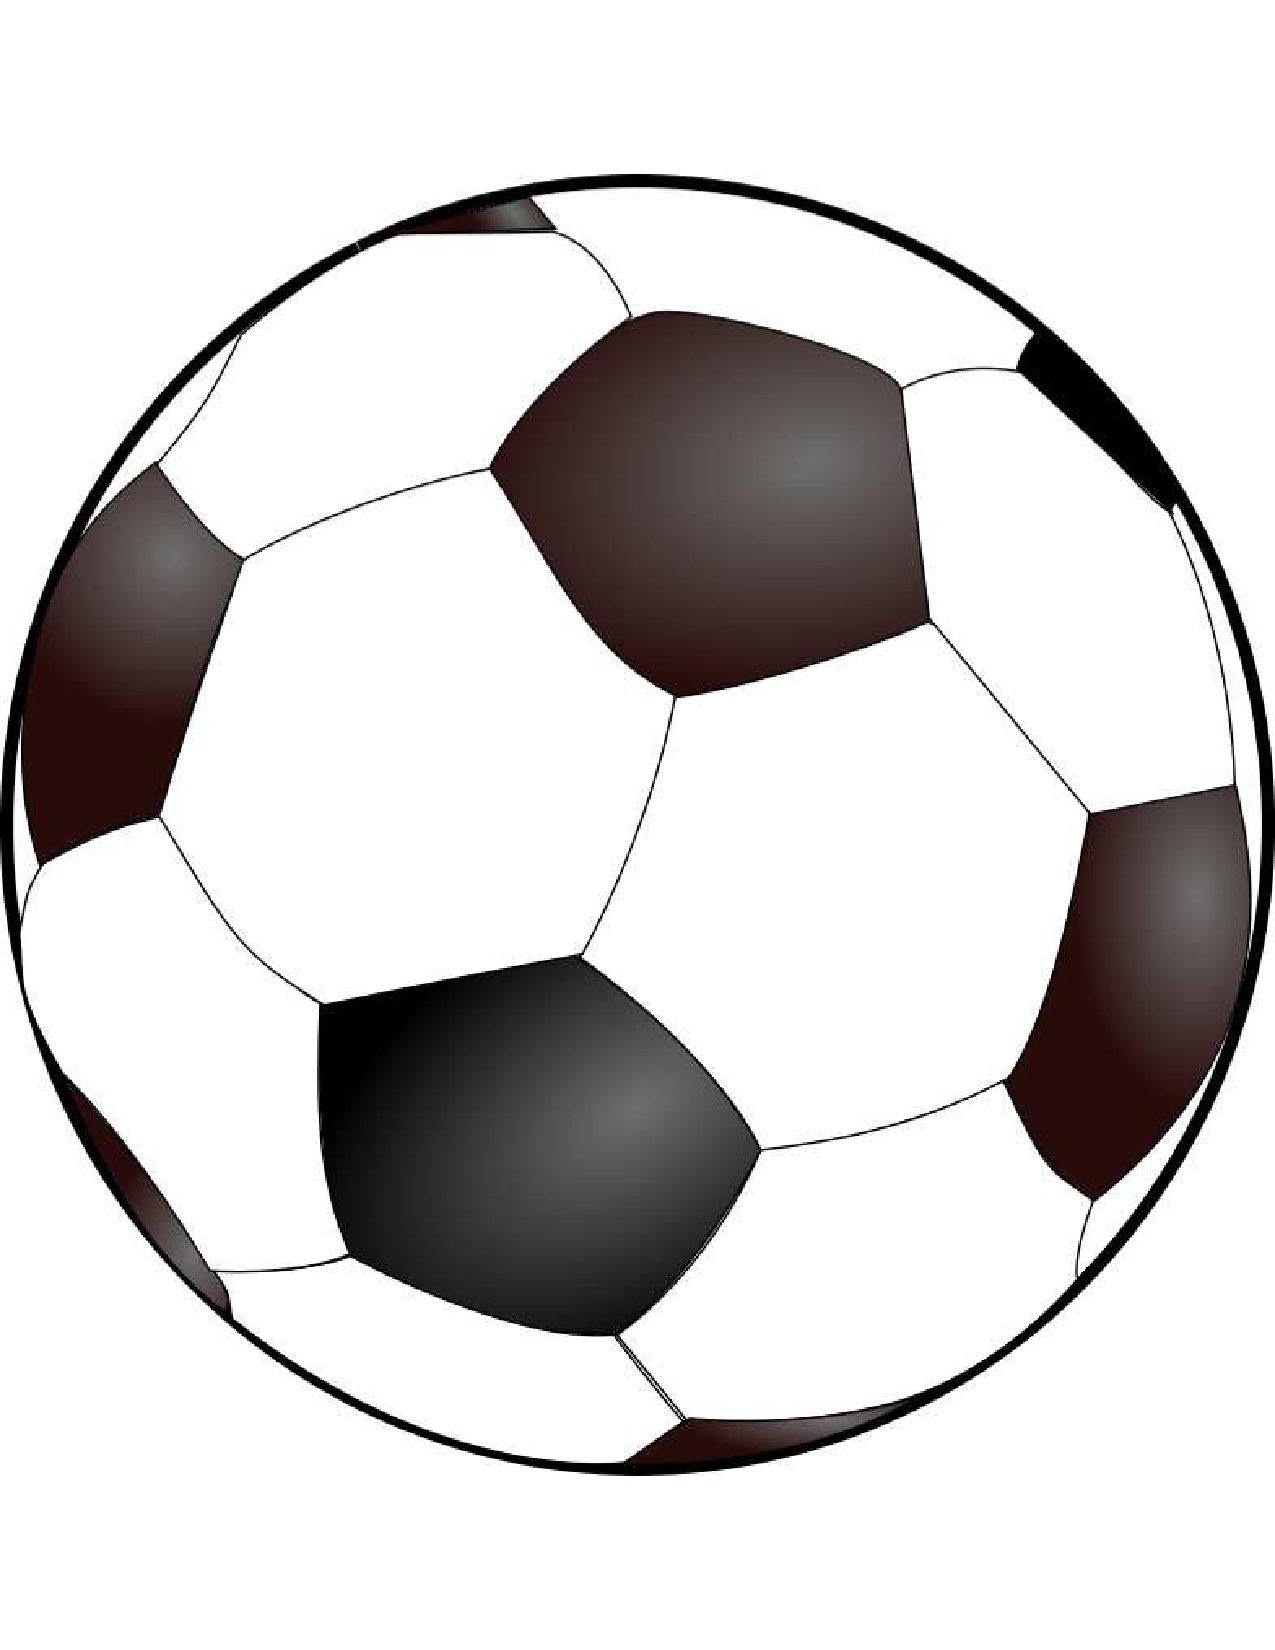
\includegraphics[scale=0.15]{ball}
	\end{minipage}
	
	
		

	%is to be made into an extremely unfair die by painting the numbers 1 to 6, one on each face. If we assume that the orientation of the numbers on each face is irrelevant, how many distinct dice can we make?\\
% To apply Burnside we need a set $X$ and group $G$ acting on $X$ such that the orbits of the action consist of indistinct dice. Thus let $X$ be the set of all possible labelings of the faces and $G$ be the group of rotations of the prism. There are clearly $6!$ possible ways to label the faces. The group of rotations is a little trickier. Consider one of the square faces. We can leave this face where it is by performing the identity of one of three rotations. Alternatively, we can swap this face with the other square face before rotating. The result is a rotation group\footnote{We don't need to know $G$ in terms of the standard lists, just its order. However, it isn't hard to see that the rotation group is isomorphic to $D_4$.} of order 8. learly the cyclic group of order 4, generated by a $90^\circ$ rotation. Every face of a labelled cuboid has a different number, thus any element of the rotation group changes every labelling, with the exception of the identity which changes nothing. Therefore
% \[\Fix(g)=\begin{cases}
%       X,&\text{if }g=e,\\ \emptyset,&\text{if }g\neq e.
%       \end{cases}\]
% It follows that the number of distinct dice is
% \[\frac{1}{\nm G}\sum_{g\in G}\nm{\Fix(g)}=\frac{6!}{8}=90.\]
% This question can also be answered very simply using combinatorics. There are $\binom{6}{2}$ choices for the pair of numbers to be painted on the square ends. Once these are chosen, there are 6 configurations of the remaining 4 numbers on the longer sides (up to rotation of the end squares). We therefore obtain $\binom{6}{2}\cdot 6=90$ distinct dice.


	\item Repeat the previous question for a regular tetrahedron.
	
	
	
	\item Suppose $G$ is a finite group with order $p^n$ where $p$ is a prime. If $x\in G$ lies in a conjugacy class with at least 2 elements, prove that the order of $\Stab(x)$ divides $p^{n-1}$. Now use the class equation to prove that $p$ divides the order of the center $Z(G)$.
% 	If $Gx$ is an orbit with at least 2 elements, then $\nm{Gx}=\frac{\nm G}{\Stab(x)}=\frac{p^n}{\Stab (x)}\ge 2\implies \nm{\Stab(x)}\le \frac 12p^n<p^n$. Since $\Stab(x)$ is a subgroup of $G$ it must have order dividing $p^n$.
% 	
% 	To finish, observe that every index $(G:\Stab(x))$ in the class equation is divisible by $p$, as is $\nm G$. We conclude that $p$ divides $\nm{Z(G)}$.

	
	\item We prove the abelian part of Cauchy's Theorem by induction on the order of $G$.
	\begin{enumerate}
	  \item Explain why the base case $\nm G=2$ is true.
	  \item Suppose $p$ divides $\nm G\ge 3$ and assume the result holds for all abelian groups of order $<\nm G$.
	  \begin{itemize}
			\item Choose any $x\neq e$; denote its order by $m=\nm{\ip x}$ (necessarily $m\ge 2$).
			\item Choose a prime $q$ dividing $m$, define $y:=x^{m/q}$ and let $H:=\ip y$.
		\end{itemize}
		Why are we done if $q=p$?
	  \item If $q\neq p$, explain why there exists a coset $zH\in \quotient GH$ of order $p$.
	  \item Prove that $z^q$ has order $p$ in $G$.
	\end{enumerate}
	
	
	
% \begin{description}
% 	\item[\normalfont\emph{Base case}: ] If $\nm G=2$, then the only suitable prime is $p=2$. Certainly $G$ has a subgroup order 2.
% 	\item[\normalfont\emph{Induction step}: ] Suppose $\nm G\ge 3$ and assume the result holds for all abelian groups of order $<\nm G$. Suppose $p$ divides $\nm G$. We make some choices:
% 	\begin{itemize}
% 		\item Choose any $x\neq e$; let its order be $m=\nm{\ip x}$ (necessarily $m\ge 2$).
% 		\item Choose some prime $q$ dividing $m$.
% 		\item Define $y:=x^{m/q}$ and let $H=\ip y$.
% 	\end{itemize} 
% 	Plainly $y$ has order $q$. If $p=q$ we are done! Otherwise, since $G$ is abelian we have $H\triangleleft G$ and can form the factor group $\quotient GH$. This has order $\frac nq<n$ and $\frac nq$ is divisible by $p$; by the induction hypothesis there exists a coset $zH$ with order $p$. In particular, $z\not\in H$ and
% 	\[z^pH=H\implies z^p\in H=\ip{y}\implies z^p=y^k=x^{\frac{mk}q}\text{ for some $k\in\Z$}\]
% 	But then\footnotemark{} $z^q\neq e$ and
% 	\[(z^q)^p=(z^p)^q=x^{mk}=e\]
% 	whence that $z^q$ has order $p$.\qedhere
% \end{description}
% 
% \footnotetext{If $z^q=e$, then $(zH)^q=z^qH=H$ so $zH$ has order 1 or $q$; not $p$.}
	
\end{enumerate}
\end{exercises}

\clearpage

\iffalse

\section{The Sylow theorems}

\emph{In this final section many of the proofs are technical and above the level of the class. They are included for completeness and interest only. Make sure you understand the statements of the theorems and how they are used before working hard on understanding the proofs.}\\

Recall Lagrange (Theorem \ref{thm:lagrange}), and how it doesn't have a converse: e.g.~$A_4$ has order 12, but no subgroup of order 6. However, the Fundamental Theorem of Finitely Generated Abelian Groups (Theorem \ref{thm:fund}) tells us everything about subgroups of finite Abelian groups. In particular Theorem \ref{thm:abelsub} says that finite Abelian groups have subgroups of every order dividing that of the order of the parent group. For finite non-Abelian groups the story is more complicated. The Sylow theorems go some way toward establishing the existence (in the non-Abelian case) and number (in both cases) of certain subgroups.

Let $G$ act on a set $X$, and suppose there are $r$ distinct orbits of $G$ on $X$ and let $x_1,\ldots,x_r$ be elements of $X$, one from each orbit. Suppose moreover that $x_1,\ldots,x_s$ are in the 1-element orbits of $G$: i.e.~$Gx_i=\{gx_i:g\in G\}=\{x_i\}$ for each $i=1,\ldots,s$. Label $X_G=\{x_1,\ldots,x_s\}$. Then, by summing the number of elements in each orbit, we have
\[\nm X=\sum_{i=1}^r\nm{Gx_i}=\nm{X_G}+\sum_{i=s+1}^r\nm{Gx_i}.\tag*{($\ast$)}\]

CLASS EQUATION

\begin{thm}{}{pmod}
Let $\nm G$ be a power of a prime $p$ and $X$ a finite set acted on by $G$. Then $\nm X\equiv\nm{X_G}\pmod p$.
\end{thm}

\begin{proof}
$\nm{Gx_i}=(G:G_{x_i})=\frac{\nm G}{\nm{G_{x_i}}}\implies \nm G=\nm{Gx_i}\nm{G_{x_i}}$. Hence the size of each orbit $\nm{Gx_i}$ divides $\nm G$ for each $i$. For $i=s+1\ldots,r$, these orbits contain more than one element, and so $\nm{Gx_i}$ is divisible by $p$ for $i=s+1\ldots,r$. Substituting into the above equation gives the result.
\end{proof}

\begin{defn}{}{}
Let $p$ be prime. $G$ is a \emph{$p$-group} if every element of $G$ has order a power of $p$.\\
A subgroup $H$ of a group $G$ is a \emph{$p$-subgroup of $G$} if it is a $p$-group in its own right.
\end{defn}

\begin{examples}{}{}
\exstart $G=\Z_8$ is a $2$-group.
\begin{enumerate}\setcounter{enumi}{1}
\item $\Z_9$ is a 3-subgroup of $\Z_{18}$ (note that $\Z_{18}$ is not a $p$-group).
\item $\Z_3\times\Z_3$ is a 3-subgroup of $\Z_3\times\Z_6$.
\item $V$ is a 2-subgroup of $S_4$.
\item $\Z_4\times\Z_4$ is a 2-subgroup of $\Z_4\times\Z_8$ (this last is \emph{also} a 2-group).
\end{enumerate}
\end{examples}

Note that $G$ need not be a $p$-group in the second part of the definition, although certainly all subgroups of $p$-groups are themselves $p$-subgroups.

For the next theorem we consider equation $(\ast)$ for the case when $X=G$ acts on itself by conjugation. In this case we have $X_G=\{g\in G:gxg^{-1}=x,\forall x\in G\}=Z(G)$, the \emph{center} of $G$ (Section \ref{sec:center}).

\begin{thm}{Cauchy}{}
Suppose that $p$ is a prime that divides the order of a finite group $G$. Then $ G$ contains an element $x$ of order $p$ and thus a subgroup $\ip x\le G$ of order $p$ (indeed $\ip x\cong\Z_p$).
\end{thm}

\begin{proof}
We argue by induction. Suppose that all groups of order $<n$ satisfy the theorem and that $\nm{G}=n$. The theorem is certainly true for $\nm{G}=2$, hence we have our initial step.

Exercise \ref*{chap:direct}.\ref{exs:abeliansubgroup} answers the question when $G$ is Abelian, so we assume $G$ to be non-Abelian. It follows that the center $Z(G)$ is a proper subgroup of $G$ ($Z(G)=G\iff G$ Abelian), and that there exists an element $x\in G$ with $x\notin Z(G)$.

Consider the isotropy subgroup (stabiliser) $G_x$ of $x$. This is a proper subgroup of $G$ since, if it were not, then $x$ would commute with everything in $G$ and thus be in the center $Z(G)$. If $p$ divides $\nm{G_x}$ for some $x\notin Z(G)$ then we're finished by the induction hypothesis, since $G_x$ is a proper subgroup of $G$ and thus of order $<n$.

If no such $\nm{G_x}$ is divisible by $p$, then $\nm{Gx}=(G:G_x)=\frac{\nm{G}}{\nm{G_x}}$ is divisible by $p$ for all $x\notin Z(G)$. Equation $(\ast)$ then says that $p$ divides $\nm{Z(G)}$. But $Z(G)$ is a proper Abelian subgroup of $G$ and so has a subgroup of order $p$ (either by the induction hypothesis, or by Theorem \ref{thm:abelsub}).

By induction we have the theorem.
\end{proof}

\begin{example}{}{}
$S_4\times \Z_{10}\times D_6$ has order $24\cdot 10\cdot 12=2^6\cdot 3^2\cdot 5$ and thus has subgroups of orders 2, 3 \& 5 by Cauchy's Theorem. It of course has subgroups of many other orders.
\end{example}


\begin{defn}{}{normalizer}
Suppose that $H\le G$ is a subgroup. The stabilizer of $H$ under the action of $G$ by conjugation is the \emph{normalizer} of $H$. Explicitly,
\[G_H=\{g\in G:gHg^{-1}=H\}=\{g\in G:ghg^{-1}\in H,\forall h\in H\}.\]
\end{defn}


Note that $G_H$ does not fix every element of the subgroup $H$, it merely keeps $H$ together while perhaps permuting its elements.\\
$G_H$ is a subgroup of $G$ (either by general principles since it is an isotropy subgroup, or by a question in the homework). Moreover, $H$ is a normal subgroup of $G_H$. It is clear that $G_H$ is the largest subgroup of $G$ having $H$ as a normal subgroup.


\begin{lemm}{}{pgroup}
If $H$ is a $p$-subgroup of $G$, then $(G_H:H)=(G:H)\pmod p$.
\end{lemm}

\begin{proof}
Let $H$ act on the set of left cosets $\mathcal L$ of $H$ in $G$ by left multiplication. I.e.~$h\cdot(gH)=(hg)H$. Clearly $\nm{\mathcal L}=(G:H)$.\\
Now let $\mathcal L_H=\{$left cosets of $H$ fixed by $H$\}. I.e.
\begin{align*}
gH\in\mathcal L_H&\iff hgH=gH,\forall h\in H\\
&\iff g^{-1}hg\in H,\forall h\in H\iff g\in G_H.
\end{align*}
Thus $\nm{\mathcal L_H}=(G_H:H)$, the number of left cosets of $H$ in $G_H$.\\
Since $H$ is a $p$-group, Theorem \ref{thm:pmod} gives $\nm{\mathcal L}\equiv\nm{\mathcal L_H}\pmod p$, and hence the result.
\end{proof}

\begin{thm}{1st Sylow theorem}{}
Let $\nm G=p^nm$ for $p$ prime, $n\ge 1$ and $m$ not divisible by $p$. Then:
\begin{enumerate}
\item $G$ contains a subgroup of order $p^i$ for every $i=1\ldots,n$.
\item Any subgroup $H\le G$ of order $p^i$ for $i=1\ldots,n-1$ is a normal subgroup of a subgroup of $G$ of order $p^{i+1}$.
\end{enumerate}
\end{thm}

\begin{proof}
We argue by induction. $G$ has a subgroup of order $p$ by Cauchy's theorem. Suppose, for the induction hypothesis, that $G$ has a subgroup $H$ of order $p^i$.

Then $(G:H)=p^{n-i}m$ is divisible by $p$. Since $H$ is a $p$-group, Lemma \ref{lemm:pgroup} says that $(G_H:H)$ is divisible by $p$. Now $H$ is a normal subgroup of $G_H$ (see above Remark) and so the factor group $G_H/H$ exists and has order divisible by $p$. By Cauchy's theorem, $G_H/H$ has a subgroup $K$ of order $p$.\\
Now let $\gamma:G_H\to G_H/H$ be the canonical homomorphism ($\gamma(g)=gH$ for $g\in G_H$). Then
\[\gamma^{-1}(K)=\{g\in G_H:\gamma(g)\in K\}\]
is a subgroup of $G_H$, and thus of $G$. Clearly $H$ is normal in $\gamma^{-1}(K)\le G_H$, and so, by the first Isomorphism Theorem,
\[\gamma^{-1}(K)/H\cong\gamma(\gamma^{-1}(K))=K.\]
Since $K$ has order $p$, and $H$ has order $p^i$, it is clear that $\gamma^{-1}(K)$ has order $p^{i+1}$. We are done.
\end{proof}

The first Sylow theorem says that given $G$ of order $p^nm$ there exists a chain of subgroups $H_i$ of order $p^i$ which are normal inside each other:
\[\{e\}\triangleleft H_1\triangleleft H_2\triangleleft\cdots\triangleleft H_n\le G.\]
Only the final subgroup inclusion need not be normal. The third Sylow theorem gives a method whereby you can often tell if the final inclusion is normal.

\begin{defn}{}{}
A \emph{Sylow $p$-group} of a group $G$ is a $p$-group of maximal size (not contained in any larger $p$-group).
\end{defn}

It is clear that the Sylow $p$-subgroups of $G$ constitute all the subgroups of $G$ of order $p^n$. Moreover, any $p$-subgroup of $G$ is necessarily contained in a Sylow $p$-subgroup of $G$ by the second part of the Theorem.

\begin{examples}{}{}
\exstart Let $G$ be a group of order $100=2^2\cdot 5^2$. By the first Sylow theorem, $G$ has at least one Sylow 5-subgroup of order 25, and at least one Sylow 2-subgroup of order 4.
\begin{enumerate}
\item 
\item Let $H$ be a group of order $1800=2^3\cdot 3^2\cdot 5^2$. Thus $H$ has at least one Sylow 2-subgroup of order 8, at least one Sylow 3-subgroup of order 9, and at least one Sylow 5-subgroup of order 25.
\end{enumerate}
\end{examples}

The second and third Sylow theorems give us information about how Sylow $p$-subgroups are related, and how many there might be of a given group.

\begin{thm}{Second Sylow theorem}{}
Any two Sylow $p$-subgroups of a finite group $G$ are conjugate.
\end{thm}

\begin{proof}
Let $P_1,P_2$ be two Sylow $p$-subgroups of $G$. Since all Sylow $p$-subgroups have the same order (for fixed $p$), we have
\[P_2=x^{-1}P_1x\iff x^{-1}yx\in P_2, \forall y\in P_1\iff yxP_2=xP_2\iff xP_2\in\mathcal L_{P_1},\]
the set of left cosets of $P_2$ fixed by the left action of $P_1$. It suffices to show that $\mathcal L_{P_1}$ is non-empty.\\
By Lemma \ref{lemm:pgroup}, $\nm{\mathcal L_{P_1}}\equiv\nm{\mathcal L}=(G:P_2)\pmod p$, where $\mathcal L$ is the set of left cosets of $P_2$ in $G$.\\
Since $(G:P_2)$ is not divisible by $p$, we have $\nm{\mathcal L_{P_1}}\neq 0$, as required.
\end{proof}

\begin{thm}{Third Sylow theorem}{}
Suppose that the prime $p$ divides the order of the finite group $G$. Then the number of Sylow $p$-subgroups of $G$ is congruent to 1 modulo $p$ and divides $\nm G$.
\end{thm}

\begin{proof}
\def\SSS{\mathcal{S}}
Let $P$ be a Sylow $p$-subgroup of $G$, and let $\SSS$ be the set of all Sylow $p$-subgroups of $G$.\\
$G$ acts on $\SSS$ by conjugation. However, all Sylow $p$-subgroups of $G$ are conjugate so that there is only one orbit of $\SSS$ under $G$. Recall Proposition \ref{prop:orbits}: we have
\[\nm{\SSS}=\nm{\text{orbit $GP$ of $P$}}=(G:G_P)=\nm{G}{\nm{G_P}}.\]
This is clearly a divisor of $\nm G$ and so the number of Sylow $p$-subgroups divides the order $G$.\\
$P$ acts on $\SSS$ by conjugation: if $x\in P$, and $Q\in\SSS$ another Sylow $p$-subgroup, then $xQx^{-1}$ is also a Sylow $p$-subgroup and thus in $\SSS$. Since $P$ is a $p$-group acting on a set $\SSS$, Lemma \ref{lemm:pgroup} implies that
\[\nm{\SSS}\equiv\nm{\SSS_P}\pmod p.\]
That is, the number of $p$-subgroups is congruent modulo $p$ to the cardinality of the set of $p$-subgroups fixed under the action of $P$.\\
Suppose $Q\in \SSS_P$. Then $xQx^{-1}=Q$ for all $x\in P$ and so $P\le G_Q$, the normalizer of $Q$. However, we also clearly have $Q\le G_Q$. We claim that $P,Q$ are Sylow $p$-subgroups of $G_Q$. For this, observe that $P,Q$ are $p$-groups and thus $p$-subgroups of $G_Q$. If they were not Sylow $p$-subgroups of $G_Q$, then they would be contained in strictly larger Sylow $p$-subgroups of $G_Q$. But $P,Q$, being Sylow $p$-subgroups of $G$, are the largest $p$-subgroups of $G$. $G_Q\le G$ says that the Sylow $p$-subgroups of $G_Q$ must be at most the same size as those of $G$.\\
By the second Sylow theorem, $P,Q$ are conjugate subgroups in $G_Q$: i.e.~$P,Q$ are conjugate by an element $y\in G_Q$. But $Q$ is a normal subgroup of $G_Q$ (see the Remarks after Defintion \ref{defn:normalizer}) and so $Q=P$. Hence $\SSS_P=\{P\}$ and so
\[\nm{\SSS}\equiv 1\pmod p.\]
The number of Sylow $p$-subgroups of $G$ is thus congruent to 1 modulo $p$.
\end{proof}

\begin{examples}{}{}
\exstart In our example where $\nm G=100$, the only divisors of $G$ are 1, 2, 4, 5, 10, 20, 25, 50 \& 100.\\
The only one of these numbers to be simultaneously congruent to 1 modulo 5 is 1 itself. There is therefore only one Sylow 5-subgroup of $G$. Since this is the only subgroup of order 25 it must be self-conjugate and thus normal.\\
Conversely, of the above string of numbers, 1, 5 and 25 are congruent to 1 modulo 2, hence there may be 1, 5 or 25 distinct Sylow 2-subgroups of $G$.\\
We now give two examples of where we can see the Sylow $p$-subgroups explicitly.
\begin{enumerate}\setcounter{enumi}{1}
\item[]\begin{enumerate}
	\item $\Z_{100}$ clearly has order 100. Its subgroups are $\Z_k$ for $k$ each of the divisors listed above. There is thus one Sylow 5-subgroup $\Z_{25}$ and one Sylow 2-subgroup $\Z_4$.
	\item $D_{50}$ also has order 100. Its single subgroup of order 25 consists of exactly half of the 50 rotations: $\Z_{25}\cong\{\rho_0,\rho_2,\ldots,\rho_{48}\}$. Here there are 25 distinct Sylow-2 subgroups, all isomorphic to the Klein 4-group $V$. Labeling the reflections $\mu_1,\ldots,\mu_{50}$, these are
	\[V_i=\{\rho_0,\rho_{25},\mu_i,\mu_{i+25}\},\quad i=1,\ldots,25.\]
	Notice that $D_{50}$ has no subgroup isomorphic to $\Z_4$ (reflections have order 2 and rotations have orders 1, 5 or 25): by the second Sylow theorem all Sylow 2-subgroups are conjugate and thus isomorphic, so we need not look for $\Z_4$ subgroups.
	\end{enumerate}

\item Now suppose that $\nm G=20=2^2\cdot 5$. The divisors of $\nm G$ are 1, 2, 4, 5, 10 and 20. There must be either 1 or 5 Sylow 2-subgroups; and 1 Sylow 5-subgroup of $G$, which is necessarily normal. Thus $G$ has a normal subgroup isomorphic to $\Z_5$. You should be able to perform a similar analysis to the previous example to see what these subgroups are in the cases where $G$ is $\Z_{20}$ and $D_{10}$.

\item Let $\nm G=225=3^2\cdot 5^2$. The divisors of $\nm G$ are 1, 3, 5, 9, 15, 25, 45, 75, 225. There must be either 1 or 25 Sylow 3-subgroups of $G$, and only one Sylow 5-subgroup (which is thus normal).

\item Let $G$ have order $pq$, where $p<q$ are distinct primes $\ge 3$. Then all proper subgroups of $G$ are isomorphic to $\Z_p,\Z_q$. More is true. $\Z_q$ is a Sylow $q$-subgroup of $G$. The third Sylow theorem states that there can only be 1, $p$ or $q$ of these, and that the number is congruent to 1 modulo $q$. If there were $p$, then $p\equiv 1\pmod q\implies p=1+\lambda q$ for some necessarily positive integer $\lambda$, which is a contradition since $p<q$. There is thus only one Sylow $q$-subgroup of $G$.\\
The other argument is false: for example if $p,q=3,7$, then $q\equiv 1\pmod p$, so there may be 1 or 7 Sylow 3-subgroups of $G$. The former yields $\Z_{21}$, while the latter yields a new group, not seen in this class.\\
In general it can be shown that if $G$ has order $pq$, where $p<q$ are any primes such that $q-1$ is not divisible by $p$, then $G\cong\Z_{pq}$. For example, the groups $\Z_{15},\Z_{33},\Z_{35}$, etc., are the only groups up to isomorphism of their given order.
\end{enumerate}
\end{examples}

\section*{Homogeneous spaces --- for interest only}

Homogeneous spaces are an application of group actions to geometry and Physics and have extremely important applications. We now know enough to be able to give a few basic examples.

A homogeneous space is, loosely, a continuous set which looks the same around every point. For example an ant sitting on the surface of a sphere cannot distinguish between directions: every direction looks the same to him. Here is a more precise definition in terms of group actions.

\begin{defn}{}{}
Let $G\times X\to X$ be a transitive action of a continuous group (for example a matrix group) on a set $X$. Then we call $X$ a \emph{homogeneous space} (or sometimes a homogeneous $G$-space) and we write $X=G/H$ where $H$ is isomorphic to the stabilizer $G_x$ for some (indeed any) $x\in X$.
\end{defn}

$G/H$ is \emph{not} a factor group: it is the set of left cosets of $H$ in $G$. Observe that $\#(G/H)=(G:G_x)=\# Gx=\nm X$ since the action is transitive. The definition doesn't depend on the choice of $x$ because all isotropy subgroups are isomorphic in $G$ when the action is transitive:
\[y=g\cdot x\implies G_y=gG_xg^{-1}\cong G_x.\]

Homogeneous spaces are extremely useful in geometry as they allow us to describe and calculate outside of vector spaces.

\begin{examples}{}{}
\exstart The orthogonal group $\rO_3(\R)$ acts transitively on the sphere $S^2\subset\R^3$. To see this, suppose that $\V v\neq\V w$ are unit vectors, then there exists a rotation about the vector $\V v\times\V w$ taking $\V v$ to $\V w$: but any rotation is an element of $\rO_3(\R)$. Moreover $\rO_3(\R)$ preserves the lengths of vectors, so it certainly preserves the sphere.

Now consider the isotropy group of the north pole $(0,0,1)\in S^2$. If $A\in\rO_3(\R)$ fixes the north pole then, by orthogonality, it must map the perpendicular (equatorial) plane to itself: i.e.\ $A\ip{\V i,\V j}=\ip{\V i,\V j}$ preserves the span of $\V i,\V j$. Since $A$ is orthogonal, it must act as an element of the orthogonal group of 1 dimension lower on the plane $\ip{\V i,\V j}$. Thus the isotropy group at the north pole is isomorphic to $\rO_2(\R)$. This is similar to an example constructed earlier.

In particular we may write
\[S^2=\rO_3(\R)/\rO_2(\R).\]
One may therefore think of maps into the sphere in terms of maps into the coset space $\rO_3(\R)/\rO_2(\R)$. This can be extremely useful when it comes to differentiating maps into the sphere, for one can use Lie theory to do calculus on the sphere without having to rely on the surrounding vector space structure.\\

The discussion can be generalized to the $n$-sphere: $S^n=\rO_{n+1}(\R)/\rO_n(\R)$.
\begin{enumerate}\setcounter{enumi}{1}
\item Projective space is an example of a homogeneous space where there is no sensible vector space in which to work. Geometry in projective space is the geometry of perspective: very important for engineers and designers of 3d-computer graphics, amongst other things. Define
\[\pr(\R^3)=\{\text{1-dimensional vector subspaces of }\R^3\}.\]
Just like for the sphere, the orthogonal group $\rO_3(\R)$ acts transitively on the set of lines through the origin. Similarly the stabilizer of a line $\ell$ contains the orthogonal group $\rO_2(\R)$ acting on the plane perpendicular to $\ell$. Moreover it also contains the orthogonal maps sending $\ell$ to itself, namely $\pm I$ on $\ell$. This is a copy of $\rO_1(\R)$. The isotropy subgroup of a line $\ell$ is therefore isomorphic to $\rO_2(\R)\times\rO_1(\R)$, and so
\[\pr(\R^3)=\rO_3(\R)/(\rO_2(\R)\times\rO_1(\R)).\]

Just as for the sphere, the above description can be generalized to cover the set of $k$-dimensional subspaces of $\R^n$ --- the so-called \emph{Grassmannian} $G_k(\R^n)$. We have
\[G_k(\R^n)=\rO_n(\R)/(\rO_k(\R)\times\rO_{n-k}(\R)).\]

Once again this description leads to the ability to do calculus in a set that is not a vector space --- there are many, many applications.
\end{enumerate}
\end{examples}

\fi